\documentclass[aspectratio=169]{beamer}
\usepackage[utf8]{inputenc}
\usepackage[T1]{fontenc}
\usepackage[french]{babel}
\usepackage{graphicx}
\usepackage{booktabs}

\usetheme{metropolis}
\metroset{block=fill}

\title{Intégration de MedVAE pour la segmentation multi-classes d'artères coronaires}
\subtitle{Une compression médicale avec perte préserve-t-elle l'information pour la segmentation ?}
\author{[Auteur]}
\institute{[Affiliation]}
\date{\today}

\begin{document}

\maketitle

\begin{frame}{Contexte et problématique}
\begin{columns}[T]
\begin{column}{0.56\textwidth}
\textbf{Tâche.} Segmentation fine des artères coronaires sur ARCADE :
\begin{itemize}
  \item 26 classes (le fond et 25 segments)
  \item structures minces, tubulaires, peu contrastées
  \item déséquilibre extrême ($\approx 95\,\%$ de fond)
\end{itemize}
\vspace{0.6em}
\textbf{Outil.} MedVAE, auto-encodeur variationnel médical pré-entraîné : compression $\times 16$ ($512^2 \to 128^2 \times 1$), mais \alert{avec perte}.
\end{column}
\begin{column}{0.44\textwidth}
\begin{block}{Deux questions}
\begin{enumerate}
  \item La compression préserve-t-elle assez d'information anatomique pour la segmentation ?
  \item Où l'intégrer : espace \textbf{latent} ou espace \textbf{pixel} ?
\end{enumerate}
\end{block}
\end{column}
\end{columns}
\end{frame}

\begin{frame}{Méthode : cinq conditions}
\begin{columns}[T]
\begin{column}{0.52\textwidth}
\small
\begin{itemize}
  \item \textbf{A} — U-Net pleine résolution (référence)
  \item \textbf{A*} — U-Net de A sur images reconstruites, \alert{sans réentraînement} (contrôle)
  \item \textbf{B} — tête légère sur le latent gelé
  \item \textbf{C} — comme B, encodeur fine-tuné sur ARCADE
  \item \textbf{D} — U-Net réentraîné sur images reconstruites
\end{itemize}
\vspace{0.6em}
\footnotesize Espace \textbf{latent} : B, C \quad ; \quad espace \textbf{pixel} : A*, D.
\end{column}
\begin{column}{0.48\textwidth}
\centering
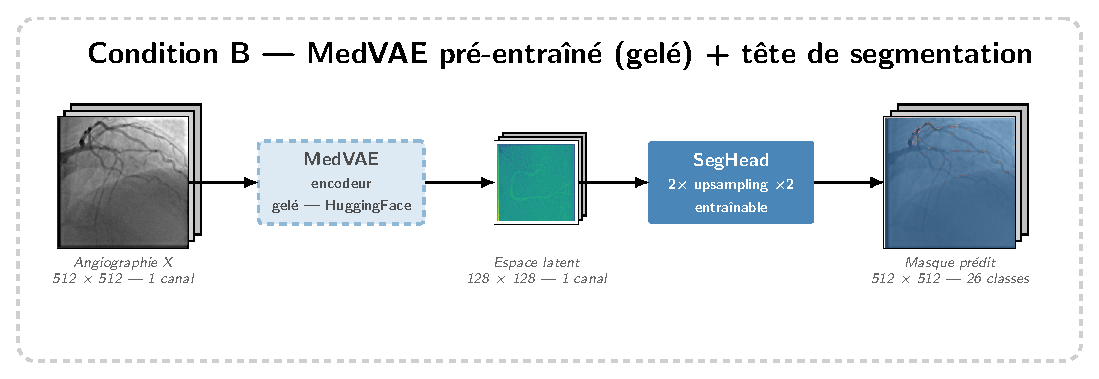
\includegraphics[width=\linewidth]{cond_B.pdf}\\[0.5em]
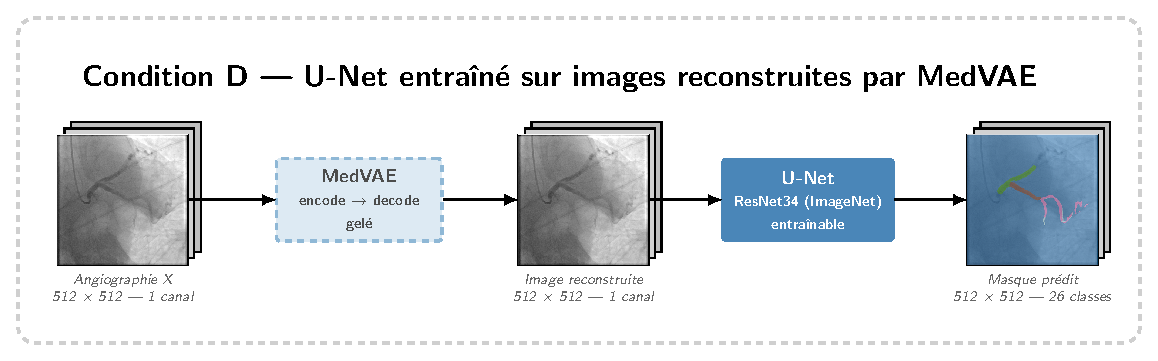
\includegraphics[width=\linewidth]{cond_D.pdf}
\end{column}
\end{columns}
\end{frame}

\begin{frame}{Résultat 1 : la segmentation depuis le latent échoue}
\begin{columns}[T]
\begin{column}{0.48\textwidth}
\begin{itemize}
  \item B et C : Dice $\approx 0{,}04$ (contre 0,433 pour A)
  \item seul le fond est prédit, IoU $\to 0$
\end{itemize}
\textbf{Pourquoi ?}
\begin{itemize}
  \item déséquilibre $95\,\%$ de fond $\Rightarrow$ minimum trivial très attracteur
  \item latent à 1 canal, \alert{aucune caractéristique multi-échelles} (ni connexions de saut)
\end{itemize}
Le fine-tuning du compresseur (C) n'y change rien.
\end{column}
\begin{column}{0.52\textwidth}
\centering
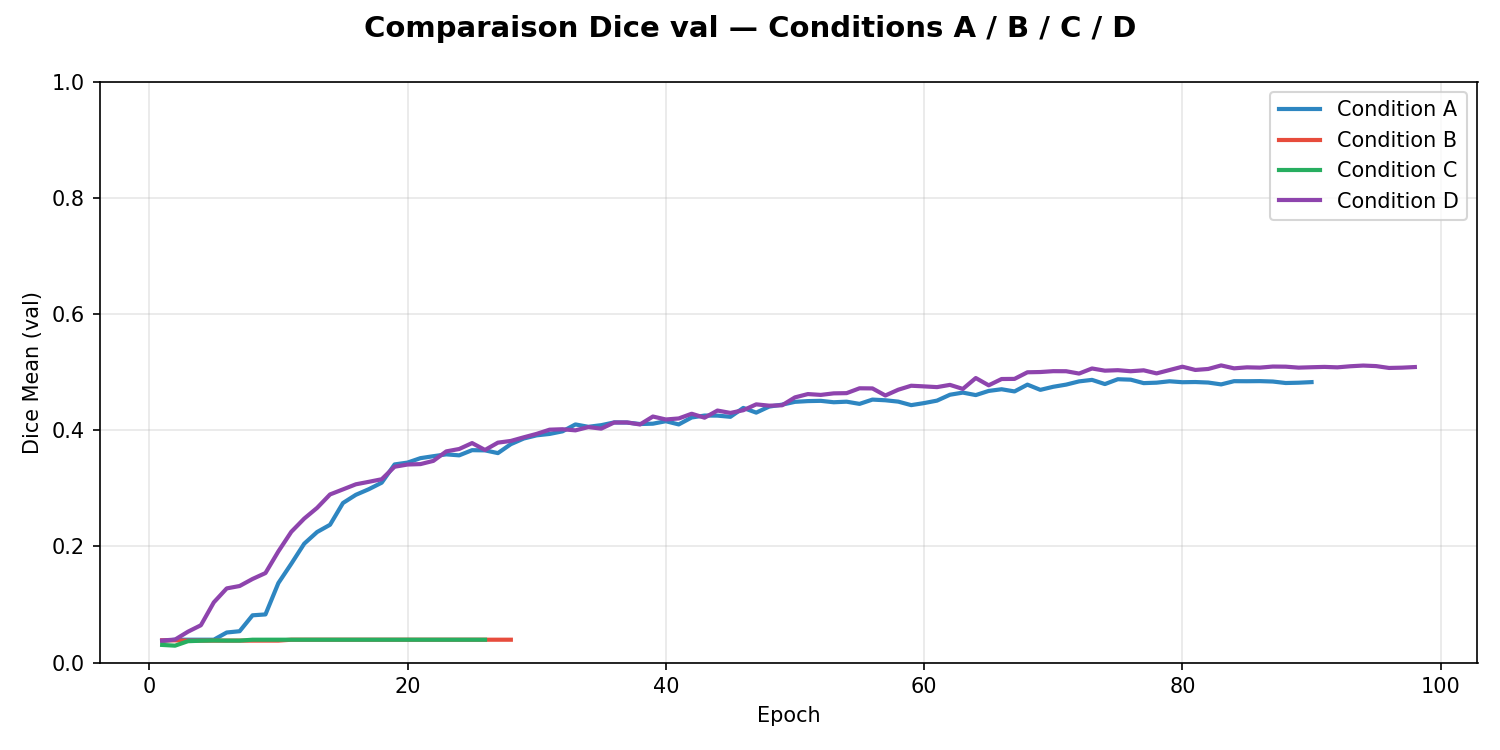
\includegraphics[width=\linewidth]{comparaison_conditions.png}
\end{column}
\end{columns}
\end{frame}

\begin{frame}{Résultat 2 : l'espace pixel préserve, l'adaptation aide}
\begin{columns}[T]
\begin{column}{0.42\textwidth}
\centering
\small
\begin{tabular}{lcc}
\toprule
Cond. & Dice & IoU \\
\midrule
A   & 0,433 & 0,499 \\
A*  & 0,434 & 0,497 \\
B   & 0,038 & 0,005 \\
C   & 0,039 & 0,000 \\
D   & \textbf{0,451} & 0,495 \\
\bottomrule
\end{tabular}
\end{column}
\begin{column}{0.58\textwidth}
\small
\begin{itemize}
  \item \textbf{Compression neutre} : A* $\approx$ A (0,434 vs 0,433)
  \item \alert{Résultat central : $D - A^{*} = +0{,}017$} \\ gain propre de l'adaptation (même entrée, seul le réentraînement diffère)
  \item gain concentré sur les segments rares et fins (C11, C18, C19)
\end{itemize}
\end{column}
\end{columns}
\vspace{-0.2em}
\centering

\includegraphics[width=0.86\textwidth]{dice_per_class.png}
\end{frame}

\begin{frame}{Prédictions qualitatives}
\vspace{0.3em}
\begin{columns}[T]
\begin{column}{0.5\textwidth}
\centering
Espace pixel : structures bien segmentées.
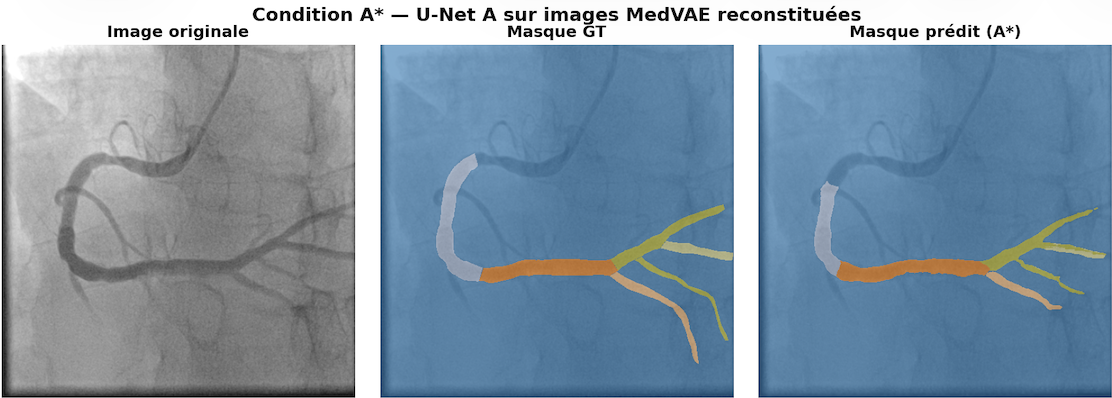
\includegraphics[width=\linewidth]{predAstar.png}\\[0.4em]
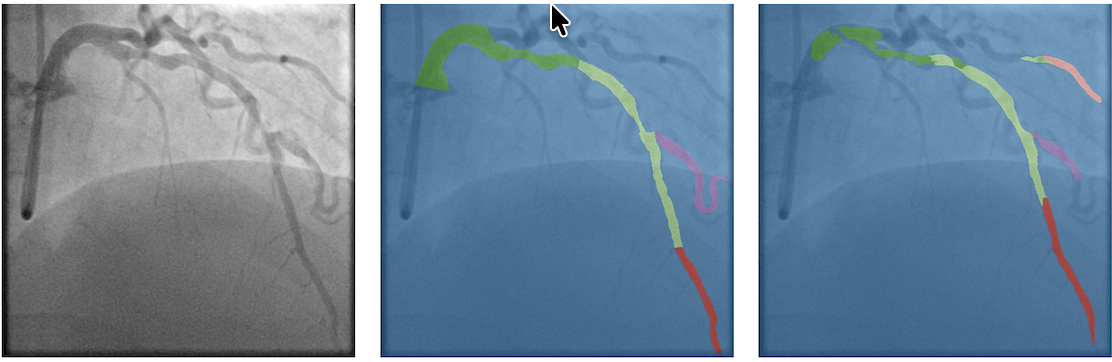
\includegraphics[width=\linewidth]{conDmieux.png}
\end{column}
\begin{column}{0.5\textwidth}
\centering
Espace latent : tout est prédit comme fond.
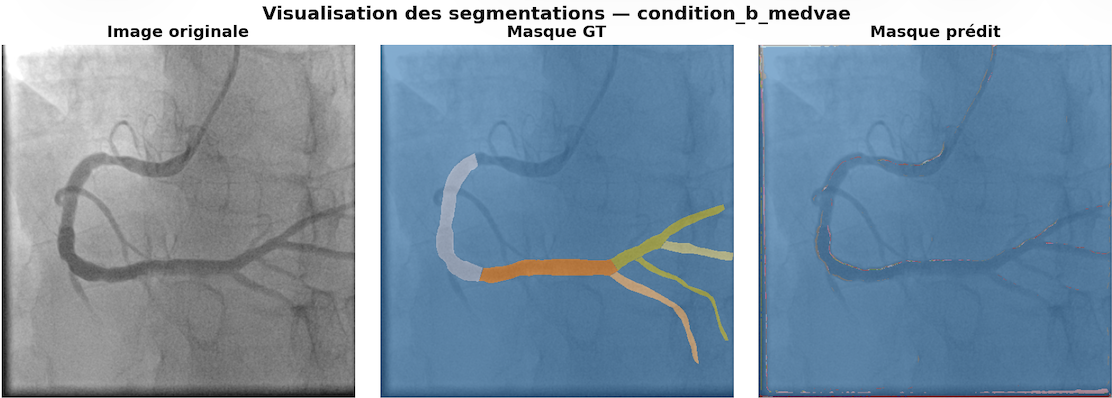
\includegraphics[width=\linewidth]{predB.png}\\[0.4em]
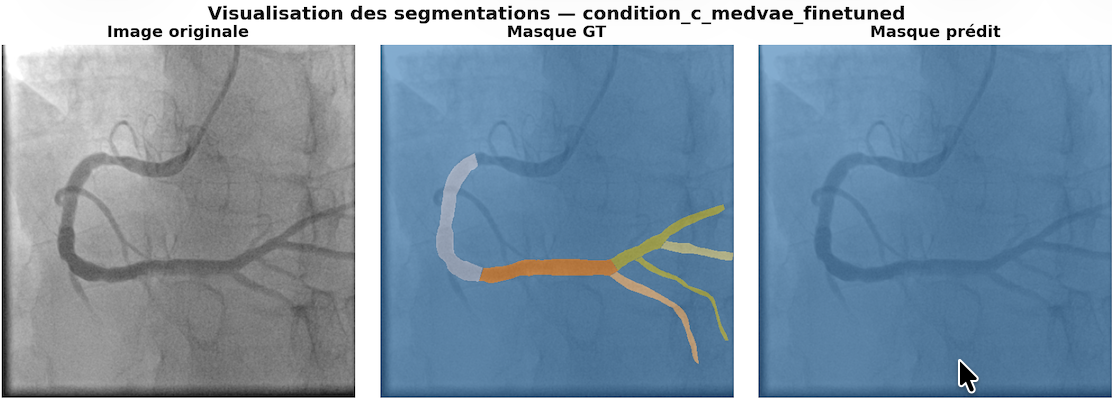
\includegraphics[width=\linewidth]{predC.png}
\end{column}
\end{columns}
\end{frame}

\begin{frame}{Conclusion}
\begin{itemize}
  \item Une compression médicale $\times 16$ \textbf{préserve} l'information pour la segmentation, mais seulement \alert{en espace pixel} (A* $\approx$ A).
  \item Le \textbf{latent} à un seul canal est \textbf{inadapté} à une tâche dense et fine ; le fine-tuning orienté reconstruction ne le débloque pas.
  \item S'adapter aux images reconstruites apporte un gain ciblé et contrôlé ($+0{,}017$), sur les structures les plus difficiles.
\end{itemize}
\end{frame}

\end{document}